\documentclass[a4paper,12pt]{article}
% Resize margins:
\usepackage[top=1.5cm, bottom=2cm, left=3cm, right=2cm]{geometry}
\usepackage{natbib} % Citation package to cite by name (use plainnat
% bib style).
\usepackage{graphicx} % Graphics.
\usepackage[labelformat=simple]{subcaption} % Get subfigure environment.
\renewcommand\thesubfigure{(\alph{subfigure})} % Reference subfigures in parentheses.
\usepackage{empheq} % Loads mathtools, which in turn loads amsmath.
\usepackage{amssymb,bm} % Maths.
\usepackage{hyperref} % Clickable links and table of contents.
\usepackage{siunitx} % SI unit package.
\usepackage{enumerate} % Labels of the 'enumerate' environment.
\graphicspath{{img/}} % Add a path to load images.
\usepackage{pgfplots} % Plots.
\pgfplotsset{width=7cm,compat=1.12} % Set size of all plots and assure 
% compatibility backwards.
\usepackage{todonotes} % Make to-do lists and visible comments.
\usepackage{tabularx, booktabs} % Tables, Commands to getter spacing above and 
% below the various rules in the table (\toprule, \bottomrule, \midrule, and 
% \cmidrule).
\usepackage{pdfpages} % Include external pdf.
\newcolumntype{Y}{>{\centering\arraybackslash}X} % Center content of the table, 
% stretching column(s) with specifier X to make table as wide as specified.

% Custom underline function:
\newcommand{\ubar}[1]{\mkern 1.5mu\underline{\mkern-1.5mu#1\mkern-1.5mu}\mkern 1.5mu}
% Double underline function:
\newcommand{\uubar}[1]{\ubar{\ubar{#1}}}
% Underline bold function:
\newcommand{\ubarbold}[1]{\ubar{\bm{#1}}}
% Double underline bold function:
\newcommand{\uubarbold}[1]{\uubar{\bm{#1}}}


\allowdisplaybreaks

\title{Computational Nonlinear Mechanics \\ \textbf{Assignment 1:\\
    Truss structure}}

\author{Rostyslav Skrypnyk\footnote{Department of Mechanics and Maritime Sciences,
    rostyslav.skrypnyk@chalmers.se}}

\date{\today}

\begin{document}

\maketitle
\tableofcontents

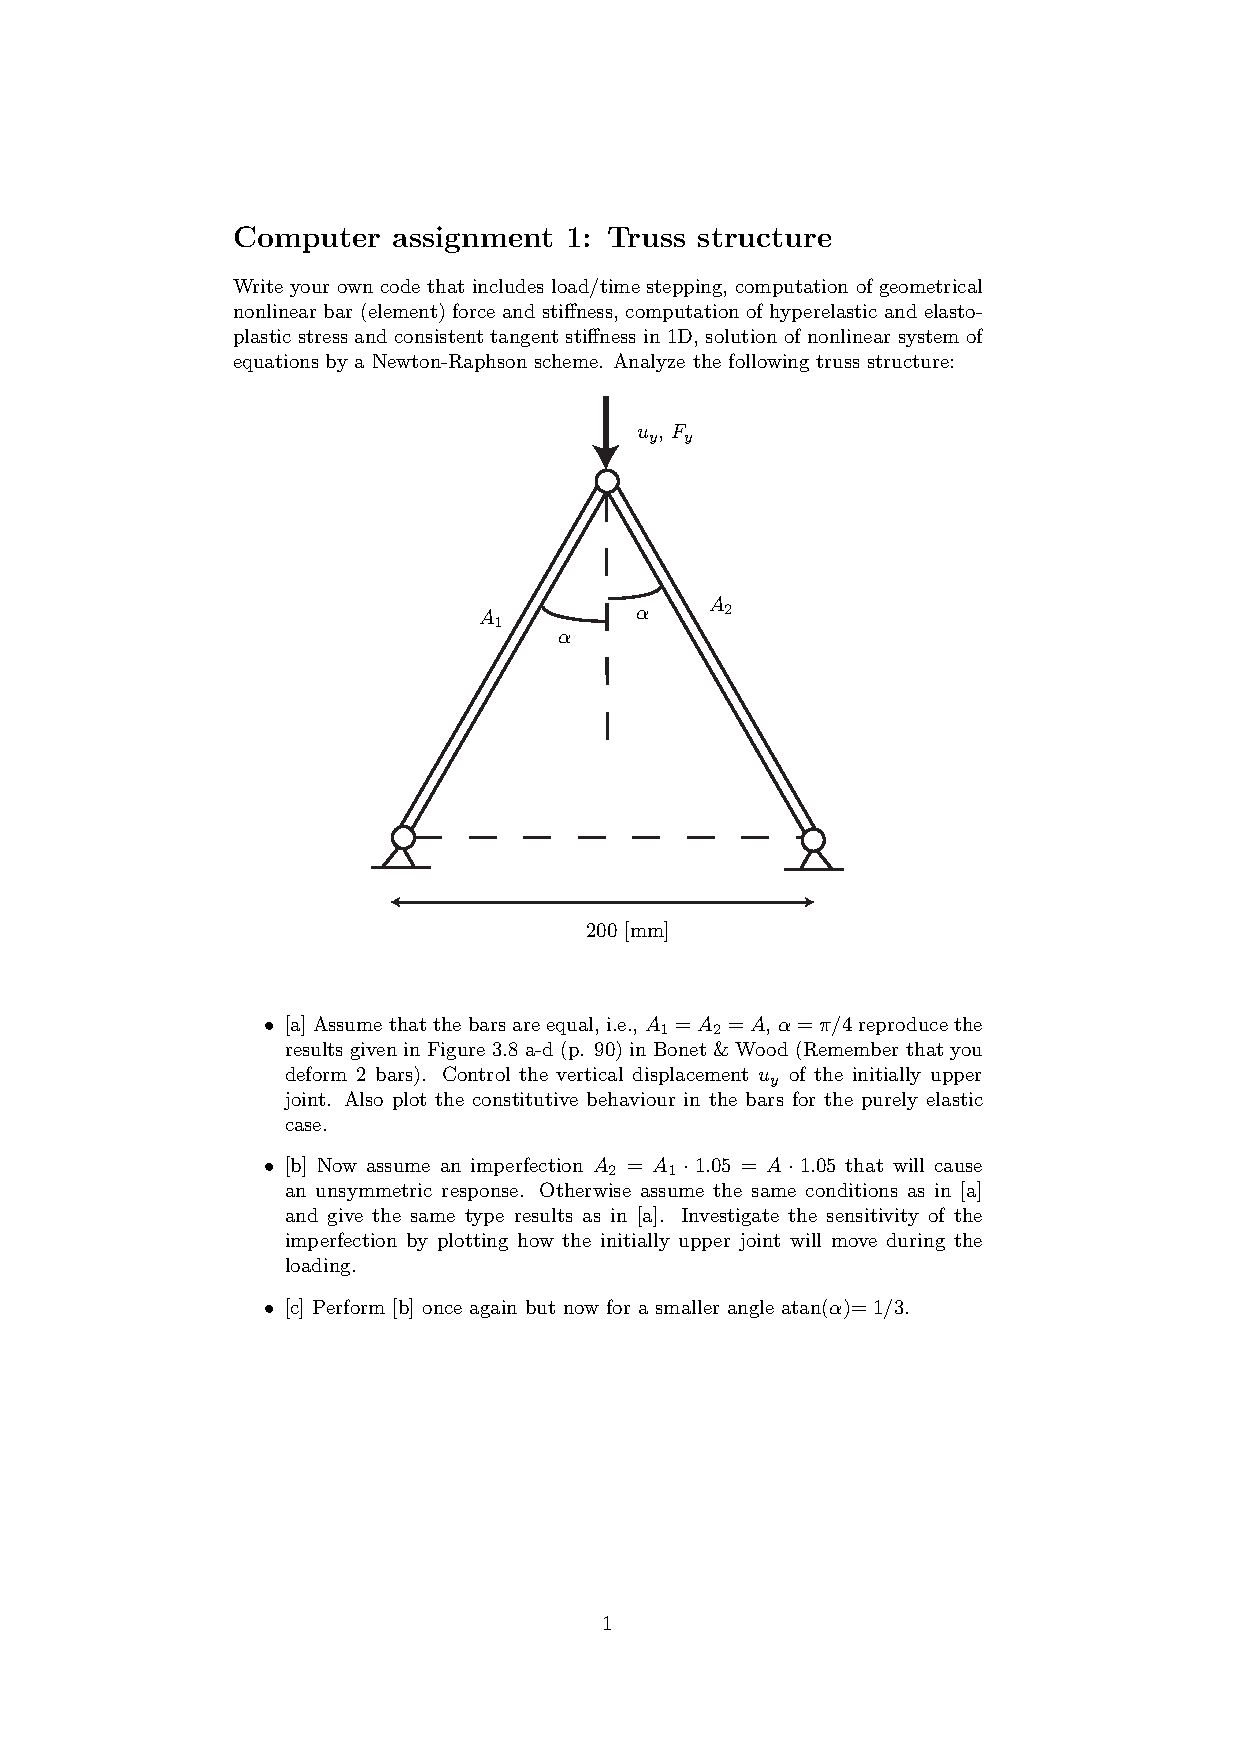
\includepdf[pages=-]{../cass1.pdf} % Task description.

\section{Theory}
\label{sec:theory}

The following is a short summary of the used equations, which were adopted
from chapter 3 of the course book~\cite{Bonet2008}.
Unless stated otherwise, the uppercase letters refer to the initial (reference)
configuration of the problem, while the lowercase ones refer to the current
configuration. The boldface letters denote vectors, matrices and tensors.

For a given load, solving the problem implies finding a configuration that
simultaneously satisfies both the global (system) equilibrium equations and
the constitutive equations.
The equilibrium equations are expressed in terms of the residual (out-of-balance)
vector \(\bm{R} (\bm{x})\) as the balance between internal and external forces:
\begin{equation}
  \bm{R} (\bm{x}) = \bm{T} (\bm{x}) - \bm{F} = \bm{0},
\end{equation}
where \(\bm{x} =\left[ \bm{x}_{1}, \bm{x}_{2}, \cdots, \bm{x}_{N} \right]^{\text{T}}\)
is the vector of current nodal positions;
\(\bm{T} =\left[ \bm{T}_{1}, \bm{T}_{2}, \cdots, \bm{T}_{N} \right]^{\text{T}}\) is
the vector of internal nodal forces;
\(\bm{F} =\left[ \bm{F}_{1}, \bm{F}_{2}, \cdots, \bm{F}_{N} \right]^{\text{T}}\) is
the vector of external nodal forces, where it is assumed to be independent
of the current nodal positions \(x\) (generally this is not true);
and \(N\) is the number of nodes.

\subsection{Hyperelasticity}
\label{sec:hyperelasticity}

In the case of hyperelastic material behaviour of a rod, i.e.\ material whose
strain energy per unit volume \(V\) does not depend on the path taken by the rod as
it moved from initial length \(L\) to the current length \(l\), the internal
truss forces \(\bm{T}_{a}\) and \(\bm{T}_{b}\) can be computed as
\begin{equation}
  \bm{T}_{b} = \frac{V E}{l} \ln \left( \frac{l}{L} \right) \bm{n}
             = \tau \frac{V}{l} \bm{n}, \quad
  \bm{T}_{a} = - \bm{T}_{b}.
\end{equation}
Here, a Young's modulus like constant \(E\) has been used to relate Kirchhoff
stress \(\tau = E \varepsilon = \sigma v / V\) to logarithmic strain
\(\varepsilon = \ln(l/L)\).

Finding equilibrium position is carried out using Newton-Raphson method, which
involves linearisation of the equilibrium equations. The linearisation yields
the directional derivative \(D \bm{T}^{(e)} (\bm{x}^{(e)}) [\bm{u}^{(e)}]\),
which gives the
expression for the tangent stiffness matrix:
\begin{equation}
  D \bm{T}^{(e)} (\bm{x}^{(e)}) [\bm{u}^{(e)}] = \bm{K}^{(e)} \bm{u}^{(e)} =
  \begin{bmatrix}
    \bm{K}_{aa}^{(e)} & \bm{K}_{ab}^{(e)} \\
    \bm{K}_{ba}^{(e)} & \bm{K}_{bb}^{(e)}
  \end{bmatrix}
  \begin{bmatrix}
    \bm{u}_{a} \\
    \bm{u}_{b}
  \end{bmatrix}
\end{equation}
with
\begin{align}
  \bm{K}_{aa}^{(e)} &= \bm{K}_{bb}^{(e)} =\left( \frac{V}{v}
                      \frac{d \tau}{d \varepsilon} \frac{a}{l} -
                      \frac{2 \sigma a}{l} \right)
                      \bm{n} \otimes \bm{n} + \frac{\sigma a}{l} \bm{I} \\
  \bm{K}_{ab}^{(e)} &= \bm{K}_{ba}^{(e)} = - \bm{K}_{aa}^{(e)},
\end{align}
where \(d \tau / d \varepsilon = E\) is the elastic material tangent modulus.

\subsection{Rate-independent plasticity}
\label{sec:plasticity}

In the case of rate-independent finite strain plasticity with isotropic hardening,
the stress is defined via elastic strain \(\varepsilon_{e}\):
\begin{align}
  \tau &= E \varepsilon_{e} = E \left( \varepsilon - \varepsilon_{p} \right) \\
  \varepsilon_{p} &= \int_{0}^{t} \dot{\varepsilon}_{p} dt \label{eq:plastic-strain}
\end{align}

The onset of plastic deformation is governed by the yield condition, which for the
problem at issue is
\begin{equation}
  f (\tau, \bar{\varepsilon}_{p}) = \left| \tau \right| - \left(
    \tau_{y}^{0} + H \bar{\varepsilon}_{p} \right) \leq 0, \quad 
  \bar{\varepsilon}_{p} \geq 0, 
\end{equation}
where \(\tau_{y}^{0}\) is the initial yield stress,
\(\bar{\varepsilon}_{p}\) is the hardening parameter and \(H\) is a material
property called plastic modulus.
At its simplest, the hardening parameter is defined as the accumulated absolute
plastic strain occurring over time:
\begin{equation}
  \bar{\varepsilon}_{p} = \int_{0}^{t} \dot{\bar{\varepsilon}}_{p} dt,
  \quad \dot{\bar{\varepsilon}}_{p} = \left| \dot{\varepsilon}_{p} \right|,
  \quad \dot{\varepsilon}_{p} = \dot{\gamma} \frac{\partial f}{\partial \tau},
\end{equation}
where \(\dot{\gamma}\) is plastic multiplier.

In a computational setting the time integration of \eqref{eq:plastic-strain} can
only be performed approximately from a finite sequence of values determined at
different time steps.
In order to satisfy the yield condition exactly at each incremental time step,
a return-mapping algorithm described in figure~\ref{fig:return-mapping} is used,
which employs incremental kinematics (see figure~\ref{fig:incr-kinematics}).
\begin{figure}[th]
  \begin{subfigure}[t]{0.38\textwidth}
    \centering
    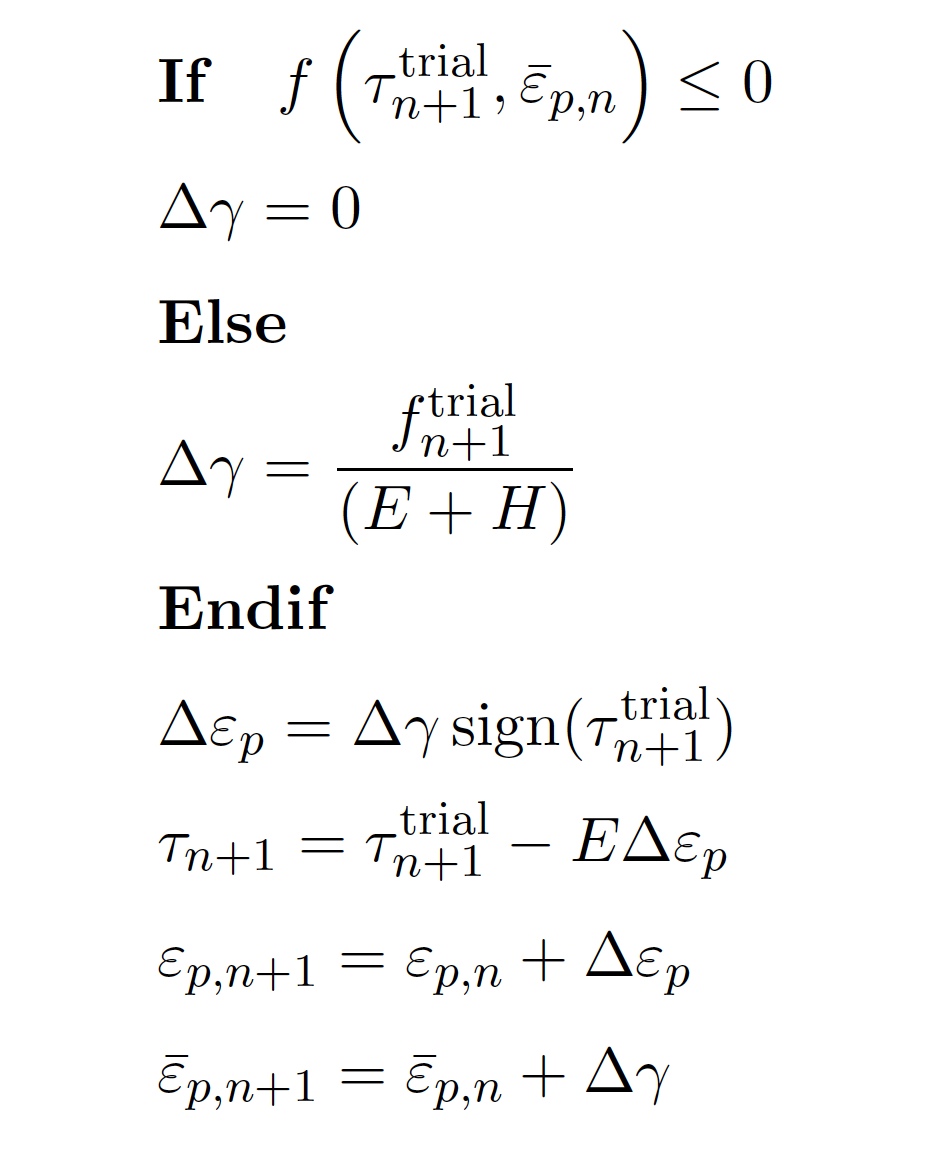
\includegraphics[width=\textwidth]{return_mapping.png}
    \caption{Return-mapping algorithm.}
    \label{fig:return-mapping}
  \end{subfigure}
  ~
  \begin{subfigure}[t]{0.56\textwidth}
    \centering
    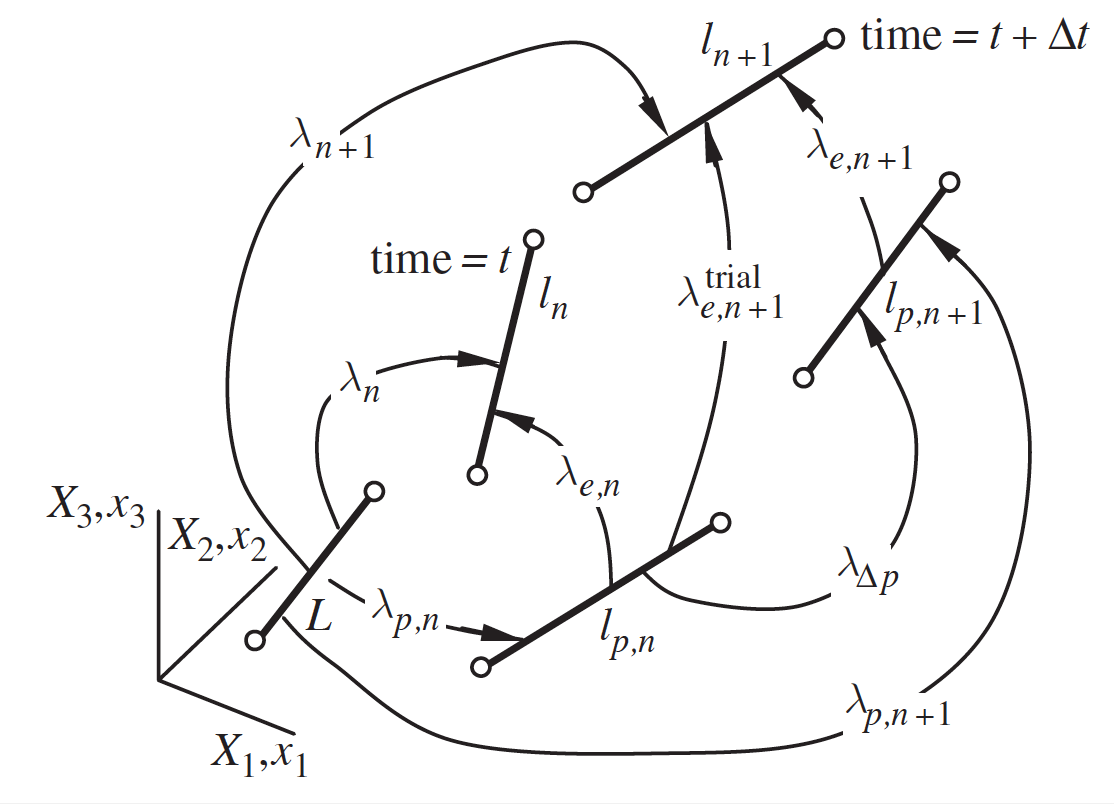
\includegraphics[width=\textwidth]{incremental_kinematics.png}
    \caption{Incremental kinematics. \(\lambda = l / L\).}
    \label{fig:incr-kinematics}
  \end{subfigure}
  \caption{Two figures from \cite{Bonet2008}.}
\end{figure}

The last matter to be addressed in the presence of plasticity is the material
tangent modulus \(d \tau / d \varepsilon\).
The tangent modulus derived from incremental considerations is generally not
the same as the one obtained from the rate equations.
The reason is that the incremental change in stress imposed by the chosen
return-mapping algorithm is different from the continuous change in stress
stemming from the rate equations.
That is why the algorithmic tangent modulus is used:
\begin{equation}
  \frac{d \tau_{n+1}}{d \varepsilon_{n+1}} = \frac{E H}{E + H}
\end{equation}
When plasticity occurs, this replaces the elastic tangent stiffness
\(d \tau / d \varepsilon = E \).

%%% Local Variables:
%%% mode: latex
%%% TeX-master: "../main"
%%% End:

\section{Task A}
\label{sec:task-a}

In the first task, the plots from \cite{Bonet2008} were reproduced.
In order to achieve that the presence of the second rod in the given
problem needed to be accounted for.
This was done by normalising the force by the total area of the two rods.
At each displacement increment, the vertical force in the top node (DOF 4)
was computed as a sum of the already acting force plus the force
needed to move the top node by the increment of the displacement,
i.e.
\begin{equation}
  F_{n+1} = F_{n} + K^{\text{global}}_{4,j} \Delta u_{j}
\end{equation}

The plots presented in figure 3.8 a-d of \cite{Bonet2008} were reproduced
and are given in figure~\ref{fig:plots-from-book}.
\begin{figure}[th]
  \centering
  % Force - deflection:
  \begin{subfigure}[t]{\textwidth}
    \begin{tikzpicture}
      \begin{axis}[
        width = 0.95\textwidth,
        height=\axisdefaultheight,
        tick label style={/pgf/number format/fixed},
        try min ticks=6,
        minor tick num=1,
        grid=both,
        xlabel = {\( (Y - y) / L \), [-]},
        ylabel = {\( F / (E A) \), [-]},
        xmin = 0, 
        xmax = 2,
        ymin = -0.15, 
        ymax = 0.2,
        legend cell align=left,
        legend style={anchor=south east, at={(1,0)}}
        ]
        \addplot+ table[skip first n=1] {data/force_deflection_elastic.dat}; % + = same automatically determined styles, but in addition it uses [options]
        \addlegendentry{elastic}
        \addplot+ table[skip first n=1] {data/force_deflection_plastic.dat};
        \addlegendentry{plastic}
      \end{axis}
    \end{tikzpicture}
    \caption{Force - deflection}
  \end{subfigure}

  % Stress - strain:
  \begin{subfigure}[t]{0.48\textwidth}
    \begin{tikzpicture}[baseline,yscale=1.0, xscale=1.0]
      \begin{axis}[
        try min ticks=7,
        minor tick num=1,
        grid=both,
        xlabel = {strain, [-]},
        ylabel = {Kirchhoff stress, [kN/mm\textsuperscript{2}]},
        xmin = -0.4, 
        xmax = 0.3,
        xtick={-0.4, -0.2, 0, 0.2},
        ymin = -30, 
        ymax = 30,
        legend cell align=left,
        legend style={anchor=south east, at={(1,0)}}
        ]
        \addplot+ table[skip first n=1] {data/stress_strain_elastic.dat};
        \addlegendentry{elastic}
        \addplot+ table[skip first n=1] {data/stress_strain_plastic.dat};
        \addlegendentry{plastic}
      \end{axis}
    \end{tikzpicture}
    \caption{Constitutive behaviour}
  \end{subfigure}
  % Total - plastic strain:
  \begin{subfigure}[t]{0.48\textwidth}
    \begin{tikzpicture}[baseline,yscale=1.0, xscale=1.0]
      \begin{axis}[
        % try min ticks=8,
        minor tick num=1,
        grid=both,
        xlabel = {total strain, [-]},
        ylabel = {plastic strain, [-]},
        xmin = -0.4, 
        xmax = 0.3,
        ymin = -0.25, 
        ymax = 0.15
        ]
        \addplot+ [mark=none] table[skip first n=1] {data/tot_pl_strain.dat};
        \addplot+  table[skip first n=1] {data/tot_pl_strain.dat}; % Plot again using style of 2nd element in cycle list.
      \end{axis}
    \end{tikzpicture}  
    \caption{Plastic - total strain}
  \end{subfigure}
  \caption{Plots of large deflection elasto-plastic behaviour from \cite{Bonet2008}.}
  \label{fig:plots-from-book}
\end{figure}


%%% Local Variables:
%%% mode: latex
%%% TeX-master: "../main"
%%% End:
 
\section{Task B}
\label{sec:task-b}

The same plots as in section~\ref{sec:task-a} were obtained for the case
when the right truss has a 5\% bigger cross-sectional area,
\(A_{2} = A_{1} \cdot 1.05\), compared to the left truss.
The plots are given in figure~\ref{fig:plots-B} for the left truss.
\begin{figure}[th]
  \centering
  % Force - deflection:
  \begin{subfigure}[t]{\textwidth}
    \begin{tikzpicture}
      \begin{axis}[
        width = 0.95\textwidth,
        height=\axisdefaultheight,
        tick label style={/pgf/number format/fixed},
        try min ticks=6,
        minor tick num=1,
        grid=both,
        xlabel = {\( (Y - y) / L \), [-]},
        ylabel = {\( F / (E A) \), [-]},
        xmin = 0, 
        xmax = 2,
        ymin = -0.15, 
        ymax = 0.2,
        legend cell align=left,
        legend style={anchor=south east, at={(1,0)}}
        ]
        \addplot+ table[skip first n=1] {data/force_deflection_elastic_B.dat}; % + = same automatically determined styles, but in addition it uses [options]
        \addlegendentry{elastic}
        \addplot+ table[skip first n=1] {data/force_deflection_plastic_B.dat};
        \addlegendentry{plastic}
      \end{axis}
    \end{tikzpicture}
    \caption{Force - deflection}
  \end{subfigure}

  % Stress - strain:
  \begin{subfigure}[t]{0.48\textwidth}
    \begin{tikzpicture}[baseline,yscale=1.0, xscale=1.0]
      \begin{axis}[
        try min ticks=7,
        minor tick num=1,
        grid=both,
        xlabel = {strain, [-]},
        ylabel = {Kirchhoff stress, [kN/mm\textsuperscript{2}]},
        xmin = -0.4, 
        xmax = 0.3,
        xtick={-0.4, -0.2, 0, 0.2},
        ymin = -30, 
        ymax = 30,
        legend cell align=left,
        legend style={anchor=south east, at={(1,0)}}
        ]
        \addplot+ table[skip first n=1] {data/stress_strain_elastic_B.dat};
        \addlegendentry{elastic}
        \addplot+ table[skip first n=1] {data/stress_strain_plastic_B.dat};
        \addlegendentry{plastic}
      \end{axis}
    \end{tikzpicture}
    \caption{Constitutive behaviour}
  \end{subfigure}
  % Total - plastic strain:
  \begin{subfigure}[t]{0.48\textwidth}
    \begin{tikzpicture}[baseline,yscale=1.0, xscale=1.0]
      \begin{axis}[
        % try min ticks=8,
        minor tick num=1,
        grid=both,
        xlabel = {total strain, [-]},
        ylabel = {plastic strain, [-]},
        xmin = -0.4, 
        xmax = 0.3,
        ymin = -0.27, 
        ymax = 0.15
        ]
        \addplot+ [mark=none] table[skip first n=1] {data/tot_pl_strain_B.dat};
        \addplot+  table[skip first n=1] {data/tot_pl_strain_B.dat}; % Plot again using style of 2nd element in cycle list.
      \end{axis}
    \end{tikzpicture}  
    \caption{Plastic - total strain}
  \end{subfigure}
  \caption{Plots of large deflection elasto-plastic behaviour of the fist truss when \(A_{2} = 1.05 A_{1}\).}
  \label{fig:plots-B}
\end{figure}

In addition, the displacement of the initially upper joint is shown in
figure~\ref{fig:node-displ}.
As could be anticipated, the joint moves in the direction of the truss with
larger cross-sectional area when that truss is stretched.
\begin{figure}[th]
  \centering
  \begin{tikzpicture}[baseline,yscale=1.0, xscale=1.0]
    \begin{axis}[
      % try min ticks=8,
      width = 0.7\textwidth,
      minor tick num=1,
      grid=both,
      xlabel = {horizontal displacement, [mm]},
      ylabel = {vertical displacement, [mm]},
      legend cell align=left,
      legend style={anchor=north east, at={(1,1)}},
      every axis plot/.append style={line width=0.8pt}, % 0.4 - default
      xmin=-12,
      xmax=30,
      ymin=-300,
      ymax=0
      ]
      \addplot+ [mark=none] table[skip first n=1] {data/node_displ_elastic_B.dat};
      \addlegendentry{elastic, \(A_{2} = 1.05 A_{1}\)}
      \addplot+ [mark=none] table[skip first n=1] {data/node_displ_plastic_B.dat};
      \addlegendentry{plastic, \(A_{2} = 1.05 A_{1}\)}
      \addplot+ [mark=none, dashed] table[skip first n=1] {data/node_displ_plastic_B_1percent.dat};
      \addlegendentry{plastic, \(A_{2} = 1.01 A_{1}\)}
      \addplot+ [mark=none, densely dotted] table[skip first n=1] {data/node_displ_plastic_B_10percent.dat};
      \addlegendentry{plastic, \(A_{2} = 1.1 A_{1}\)}
    \end{axis}
  \end{tikzpicture}
  \caption{Displacement of the initially upper node of the first (left) truss.}
  \label{fig:node-displ}
\end{figure}

%%% Local Variables:
%%% mode: latex
%%% TeX-master: "../main"
%%% End:

\section{Task C}
\label{sec:task-c}

The same plots as in section~\ref{sec:task-b} were obtained for the case
when the truss angle \(\alpha = \operatorname{atan} (1/3)\).
The plots are given in figure~\ref{fig:plots-C} for the left truss.
\begin{figure}[th]
  \centering
  % Force - deflection:
  \begin{subfigure}[t]{\textwidth}
    \begin{tikzpicture}
      \begin{axis}[
        width = 0.95\textwidth,
        height=\axisdefaultheight,
        tick label style={/pgf/number format/fixed},
        try min ticks=6,
        minor tick num=1,
        grid=both,
        xlabel = {\( (Y - y) / L \), [-]},
        ylabel = {\( F / (E A) \), [-]},
        xmin = 0, 
        xmax = 2,
        ymin = -0.15, 
        ymax = 0.2,
        legend cell align=left,
        legend style={anchor=south west, at={(0,0)}}
        ]
        \addplot+ table[skip first n=1] {data/force_deflection_elastic_C.dat}; % + = same automatically determined styles, but in addition it uses [options]
        \addlegendentry{elastic}
        \addplot+ table[skip first n=1] {data/force_deflection_plastic_C.dat};
        \addlegendentry{plastic}
      \end{axis}
    \end{tikzpicture}
    \caption{Force - deflection}
  \end{subfigure}

  % Stress - strain:
  \begin{subfigure}[t]{0.48\textwidth}
    \begin{tikzpicture}[baseline,yscale=1.0, xscale=1.0]
      \begin{axis}[
        try min ticks=5,
        minor tick num=1,
        grid=both,
        xlabel = {strain, [-]},
        ylabel = {Kirchhoff stress, [kN/mm\textsuperscript{2}]},
        % xmin = -0.4, 
        xmax = 0.4,
        % xtick={-0.4, -0.2, 0, 0.2},
        % ymin = -30, 
        % ymax = 30,
        legend cell align=left,
        legend style={anchor=south east, at={(1,0)}}
        ]
        \addplot+ table[skip first n=1] {data/stress_strain_elastic_C.dat};
        \addlegendentry{elastic}
        \addplot+ table[skip first n=1] {data/stress_strain_plastic_C.dat};
        \addlegendentry{plastic}
      \end{axis}
    \end{tikzpicture}
    \caption{Constitutive behaviour}
  \end{subfigure}
  % Total - plastic strain:
  \begin{subfigure}[t]{0.48\textwidth}
    \begin{tikzpicture}[baseline,yscale=1.0, xscale=1.0]
      \begin{axis}[
        tick label style={/pgf/number format/fixed},
        % try min ticks=8,
        minor tick num=1,
        grid=both,
        xlabel = {total strain, [-]},
        ylabel = {plastic strain, [-]},
        % xmin = -0.4, 
        % xmax = 0.2,
        % ymin = -0.1, 
        ymax = 0.01
        ]
        \addplot+ [mark=none] table[skip first n=1] {data/tot_pl_strain_C.dat};
        \addplot+  table[skip first n=1] {data/tot_pl_strain_C.dat}; % Plot again using style of 2nd element in cycle list.
      \end{axis}
    \end{tikzpicture}  
    \caption{Plastic - total strain}
  \end{subfigure}
  \caption{Plots of large deflection elasto-plastic behaviour of the fist truss when \(A_{2} = 1.05 A_{1}\).}
  \label{fig:plots-C}
\end{figure}

In addition, the displacement of the initially upper joint is shown in
figure~\ref{fig:node-displ-C}.
It is evident that for such small angle the solution is sensitive to the
difference in cross-section area between the trusses.
\begin{figure}[th]
  \centering
  \begin{tikzpicture}[baseline,yscale=1.0, xscale=1.0]
    \begin{axis}[
      % try min ticks=8,
      width = 0.7\textwidth,
      minor tick num=1,
      grid=both,
      xlabel = {horizontal displacement, [mm]},
      ylabel = {vertical displacement, [mm]},
      legend cell align=left,
      legend style={anchor=center, at={(0.5,0.5)}},
      every axis plot/.append style={line width=0.8pt}, % 0.4 - default
      % xmin=-12,
      % xmax=30,
      % ymin=-300,
      ymax=0
      ]
      \addplot+ [mark=none] table[skip first n=1] {data/node_displ_elastic_C.dat};
      \addlegendentry{elastic, \(A_{2} = 1.05 A_{1}\)}
      \addplot+ [mark=none] table[skip first n=1] {data/node_displ_plastic_C.dat};
      \addlegendentry{plastic, \(A_{2} = 1.05 A_{1}\)}
      \addplot+ [mark=none, dashed] table[skip first n=1] {data/node_displ_plastic_C_1percent.dat};
      \addlegendentry{plastic, \(A_{2} = 1.01 A_{1}\)}
      \addplot+ [mark=none, densely dotted] table[skip first n=1] {data/node_displ_plastic_C_10percent.dat};
      \addlegendentry{plastic, \(A_{2} = 1.1 A_{1}\)}
    \end{axis}
  \end{tikzpicture}
  \caption{Displacement of the initially upper node of the first (left) truss.}
  \label{fig:node-displ-C}
\end{figure}

Obtaining the convergence for this task was the most problematic.
Even in the case of elastic material response, a situation depicted
in the figure~\ref{fig:no-newton} was occurring, where the local
minimum prevented the Newton-Raphson method from finding the
correct solution.
In those situations, the false position method was used instead.
\begin{figure}[th]
  \centering
  \begin{tikzpicture}[baseline,yscale=1.0, xscale=1.0]
    \begin{axis}[
      try min ticks=7,
      width = 0.7\textwidth,
      minor tick num=1,
      grid=both,
      xlabel = {displacement, [mm]},
      ylabel = {residual, [N]},
      ]
      \addplot+ table[skip first n=1] {data/residual_vs_du.dat};
    \end{axis}
  \end{tikzpicture}
  \caption{Example of situation, where Newton-Raphson method can fail.}
  \label{fig:no-newton}
\end{figure}


%%% Local Variables:
%%% mode: latex
%%% TeX-master: "../main"
%%% End:

\section{Matlab code}
\label{app:matlab-code}

The Matlab code can be found in the Git repository on
\href{https://github.com/iamrosk/nonlinear-truss.git}{Github}.

%%% Local Variables:
%%% mode: latex
%%% TeX-master: "../main"
%%% End:


\bibliographystyle{abbrv}
\bibliography{references}

\end{document}

%%% Local Variables:
%%% mode: latex
%%% TeX-master: t
%%% End:
